\chapter*{Introduction}
\addcontentsline{toc}{chapter}{Introduction}
\markboth{Introduction}{Introduction}
\label{chap:introduction}
%\minitoc

\setlength{\parskip}{0.7pt}


\section*{Contexte}
    \paragraph{}Dans le cadre du Cursus Master en Ingénierie de 3ème année de licence informatique, nous ---~Victor \textsc{Huesca} et Jérémie \textsc{Dautheribes} --- avons entamé la réalisation d'un réseau de capteurs pour superviser un élevage de lémuriens. Cet élevage se situe à l'animalerie de la Faculté des Sciences de Montpellier. Les lémuriens étudiés ont la particularité d'avoir un cycle de vie plus court que la plupart de leurs congénères, que permet d'étudier plus rapidement les effets de la maladie d'Alzheimer. 
    
    \paragraph{}Ce projet annuel est encadré par M. Éric \textsc{Bourreau}, chercheur au Laboratoire d'Informatique, de Robotique et de Micro-électronique de Montpellier (LIRMM) au sein de l'équipe Méthodes Algorithmes pour l'Ordonnancement et les Réseaux (MAORE). Son objectif est le déploiement d'un déployer un réseau de capteurs sans fil pour récolter diverses informations sur l'environnement des lémuriens. Ce projet se réalisant sur un an, la première partie est donc plutôt orientée sur l'étude des différentes possibilités : elle s'intéresse aux différentes informations que nous pouvons recueillir sur l'environnement des lémuriens, le matériel à notre disposition, son installation et son amélioration si nécessaire. Elle s'intéresse également aux divers scénarios de déploiement des capteurs à l'intérieur et autour de l'animalerie. Il s'agit donc d'une étude préalable à l'installation concrète, sur la faisabilité, sur les différentes possibilités de déploiement, les technologies et matériels pouvant être utilisés, etc. 
    
    \paragraph{}Les diverses informations recueillies par les capteurs seront transmises à un serveur. Celui-ci hébergera un site web sur lequel il sera possible de visualiser des statistiques liées aux informations recueillies sur l'environnement des lémuriens (comme la température, le taux d'humidité, etc.). Le cahier des charges vis-à-vis du site web n'est pas fixé et des fonctionnalités supplémentaires pourront faire leur apparition en fonction des possibilités données par les capteurs. Ce rapport s'intéresse donc principalement au réseau de capteurs et aux technologies reliées à ce sujet. 

\clearpage
\section*{Internet des Objets}
    \paragraph{}Ce projet s'inscrit dans l'évolution d'Internet et du web que connaît notre société actuellement et qui est appelée << Internet des Objets >> (IdO) ou plus connu sa désignation anglaise << Internet of Things >> (IoT). Cette évolution d'Internet consiste à interconnecter toujours plus d'objets de diverses natures pour avoir des systèmes toujours intelligents et automatisés et qui est responsable en partie de l'explosion du volume d'échange de données sur les réseaux de ces dernières années. Les applications de cette technologie sont donc diverses et variées. On trouve par exemple les maisons connectées \textit{(cf. figure \ref{fig:maison})} qui permettent de gérer à distance (par son smartphone par exemple) diverses fonctionnalités comme l'ouverture et la fermeture des volets et de la porte, le chauffage, la lumière, les systèmes audios et vidéos\dots
    
    \begin{figure}[h]
        \centering
        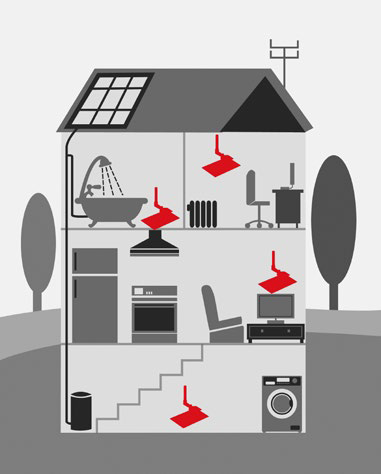
\includegraphics[scale=0.7]{images/photos/maison-connecte.png}
        \caption{Schéma d'une maison connectée selon Libelium \textit{(cf. chapitre \ref{chap:etat-art})}}
        \label{fig:maison}
    \end{figure}
    
    \paragraph{}Mais aussi les villes connectées ou \emph{Smart City} avec la gestion automatique de l'éclairage public, la surveillance vidéo et audio et autres processus intelligents et connectés. Cette évolution a été rendue possible par la miniaturisation des technologies et l'évolution toujours plus importante de la puissance de calcul. Il est donc aujourd'hui possible d'avoir des appareils qui prennent peu de place et qui possèdent une puissance de calcul suffisante pour effectuer de nombreuses tâches autrefois impossibles sur de si petits appareils.

    \paragraph{}Les smartphones sont considérés comme étant les premiers objets à avoir lancé l'IoT. Ils sont depuis peu rejoints par toutes sortes d'objets et réseaux. À ces objets sont connectés divers capteurs de lumière, de température, de présence, d'humidité, de concentration de CO$_{2}$, d'O$_{2}$, etc. Ces capteurs ne sont pas de réelles nouveautés en eux-mêmes, mais leur miniaturisation a permis de les intégrer à des objets plus petits et ainsi de favoriser leur développement chez les industriels et les particuliers. Selon l'ETH de Zurich \cite{eth}, entre 2015 et 2025 plus de 150 milliards d'objets devraient se connecter entre eux ; à l'horizon 2020 le marché devrait atteindre une valeur de 7\,100 milliards d'euros \cite{marche}. En France, des tests ont été réalisés dans plusieurs villes, comme dans la banlieue de Lyon par exemple qui a expérimenté des lampadaires ne s'allumant qu'en détectant la présence de piétons ou de véhicules \cite{monde}. 

    \paragraph{}C'est donc un marché particulièrement lucratif et dans lequel de nombreuses entreprises se sont lancées. C'est le cas de la société espagnole Libelium qui est le fournisseur du matériel dont nous disposons. Elle a été fondée en 2006 suite à la scission de l'Université de Saragosse. Elle est impliquée dans de nombreux projets de réseau de capteurs, notamment SmartSantander (\emph{Smart City} testée dans plusieurs villes européennes) qui utilise plusieurs centaines de capteurs Libelium \cite{santander}.
